\PassOptionsToPackage{indonesian}{babel}
\PassOptionsToPackage{table}{xcolor}
\documentclass{fairmeta}

\usepackage[utf8]{inputenc}
\usepackage{amsmath}
\usepackage{pgfplots}
\usepackage{tabularx}
\usepackage{longtable}
\usepackage{array}
\usepackage{listings}
\usepackage{xurl}
\usetikzlibrary{arrows.meta,positioning,fit,calc,backgrounds}

\definecolor{fairamber}{HTML}{E29400}
\pgfplotsset{
  compat=1.18,
  every axis/.append style={
    font=\small,
    axis line style={draw=metafg!55},
    tick style={draw=metafg!55},
    major grid style={draw=metafg!20,densely dotted},
    legend style={draw=none,fill=none,font=\small},
    line width=1.2pt
  }
}
\selectlanguage{indonesian}
\addto\captionsindonesian{%
  \renewcommand{\contentsname}{Daftar Isi}%
  \renewcommand{\listfigurename}{Daftar Gambar}%
  \renewcommand{\listtablename}{Daftar Tabel}%
  \renewcommand{\figurename}{Gambar}%
  \renewcommand{\tablename}{Tabel}%
}
\setcounter{secnumdepth}{2}
\setcounter{tocdepth}{2}
\emergencystretch=2em
\renewcommand{\arraystretch}{1.12}
\captionsetup[table]{skip=5pt}
\captionsetup[figure]{skip=6pt}


\newcolumntype{L}[1]{>{\raggedright\arraybackslash}p{#1}}
\newcolumntype{R}[1]{>{\raggedleft\arraybackslash}p{#1}}
\newcolumntype{Y}{>{\raggedright\arraybackslash}X}
\newcommand{\code}[1]{\texttt{\detokenize{#1}}}
\newtcolorbox{evidencebox}[1]{
  enhanced,breakable,
  colback=metabg,
  frame hidden,
  borderline west={2pt}{0pt}{metablue},
  arc=2mm,
  left=2.5mm,right=2.5mm,top=1.5mm,bottom=1.5mm,
  before skip=0.8em,after skip=0.8em,
  title={#1},
  fonttitle=\sffamily\bfseries\color{metafg},
  attach boxed title to top left={xshift=1.5mm,yshift=-1mm},
  boxed title style={colback=metabg,frame hidden}
}
\lstset{
  basicstyle=\ttfamily\footnotesize,
  columns=fullflexible,
  keepspaces=true,
  breaklines=true,
  frame=none,
  backgroundcolor=\color{metabg},
  xleftmargin=0.4em,
  aboveskip=0.3em,
  belowskip=0.3em
}
\newcommand{\eraserlink}[1]{%
  \par\smallskip{\footnotesize Versi interaktif: \href{#1}{buka diagram di Eraser}.}\par
}

\makeatletter
\renewcommand{\mymaketitle}{%
  \thispagestyle{empty}%
  \tcbset{enhanced,frame hidden}%
  \tcbset{left=0.5cm,right=0.5cm,top=0.5cm,bottom=0.5cm,arc=10pt}%
  \tcbset{colback=metabg,before skip=0pt,grow to left by=1.5pt,grow to right by=1.5pt}%
  \tcbset{overlay={\node[anchor=north east,at=(frame.north east),
    xshift=-0.5cm,yshift=-0.45cm,fill=metafg,rounded corners=3pt,inner sep=5pt]
    {
\includegraphics[width=2.25cm]{assets/stei-logo.png}};}}%
  \begin{tcolorbox}
    \setlength{\parindent}{0cm}%
    \setlength{\parskip}{0.5cm}%
    {\setlength{\parskip}{0cm}%
      \raggedright\nohyphens%
      {\setstretch{1.35}\parbox{\dimexpr\linewidth-3.3cm\relax}{\titlelist}\par}%
      \vskip 0.2cm%
      \authorlist\par%
      \vskip 0.2cm%
      \affiliationlist\par%
      \contributionlist\par%
    }%
    \abstractlist\par%
    \vskip 0.5cm%
    {\setlength{\parskip}{0cm}%
      \ifdefempty{\metadatalist}{\vspace*{0.65cm}}{\metadatalist\par}%
    }%
  \end{tcolorbox}%
  \tcbset{reset}%
  \FloatBarrier
}
\makeatother

\title{Arsitektur Layanan Terdistribusi untuk Koordinasi Data Kebencanaan}
\author[1]{Benedict Presley (13523067)}
\author[1]{Muhammad Fathur Rizky (13523105)}
\author[1]{Ahmad Wicaksono (13523121)}
\affiliation[1]{Program Studi Teknik Informatika, Sekolah Teknik Elektro dan Informatika, Institut Teknologi Bandung}
\metadata[Tanggal]{25 September 2026}
\metadata[Kelompok]{SidequestProxy}
\metadata[Mata kuliah]{IF4031 Arsitektur Aplikasi Terdistribusi, Milestone 1}
\metadata[Email]{\email{13523067@std.stei.itb.ac.id};\ \email{13523105@std.stei.itb.ac.id};\ \email{13523121@std.stei.itb.ac.id}}
\abstract{Koordinasi informasi kebencanaan menuntut integrasi sumber data yang otonom, respons layanan yang tidak seragam, dan distribusi informasi kepada beberapa konsumen. Makalah ini menyajikan rancangan dan evaluasi prototipe yang menghubungkan layanan simulasi Badan Meteorologi, Klimatologi, dan Geofisika (BMKG) serta Pusat Vulkanologi dan Mitigasi Bencana Geologi (PVMBG) melalui komponen koordinasi Badan Nasional Penanggulangan Bencana (BNPB). Aggregator mengambil data melalui REST, menyimpannya sebagai HazardEvent kanonik pada PostgreSQL, dan mempertahankan atribut tambahan dalam JSONB. Komunikasi internal menggunakan gRPC, sedangkan transaksi outbox dan RabbitMQ memisahkan penyimpanan kejadian dari distribusinya. Evaluasi lokal mencakup pemetaan data, perubahan skema aditif, isolasi keterlambatan sumber, otorisasi, pembangunan ulang layanan, dan pemulihan antrean. Dalam uji isolasi 25 pengguna virtual per sumber selama 30 detik, persentil ke-95 (p95) pembacaan BMKG melalui Client API mencapai 8,790 ms ketika penundaan polling PVMBG dikonfigurasi hingga 3 detik. Uji berkelanjutan 50 pengguna virtual selama 60 detik menghasilkan 28.211 permintaan, p95 13,970 ms, dan tingkat kesalahan 0\%. Hasil tersebut berlaku untuk konfigurasi lokal yang diuji; deduplikasi konsumen belum bertahan setelah proses dimulai ulang.\\[0.6em]\textbf{Kata kunci:} sistem terdistribusi, interoperabilitas data, evolusi skema, otorisasi, transactional outbox, pengujian beban.}
\hypersetup{pdftitle={Arsitektur Layanan Terdistribusi untuk Koordinasi Data Kebencanaan},pdfauthor={Benedict Presley; Muhammad Fathur Rizky; Ahmad Wicaksono}}

\begin{document}
\selectlanguage{indonesian}

\hypersetup{pageanchor=false}
\maketitle
\clearpage
\pagenumbering{roman}
\hypersetup{pageanchor=true}

\section*{Identitas Kelompok dan Kontribusi}
\addcontentsline{toc}{section}{Identitas Kelompok dan Kontribusi}

\textbf{Nama kelompok:} SidequestProxy. Nama dan NIM anggota tercantum pada halaman sampul. Rincian kontribusi pada Tabel~\ref{tab:contributions} masih menunggu konfirmasi seluruh anggota sebelum pengumpulan.

\begin{table}[htbp]
\centering
\small
\caption{\textbf{Kontribusi anggota menunggu konfirmasi kelompok.} Tiga kegiatan mengikuti ketentuan laporan M1.}
\label{tab:contributions}
\begin{tabularx}{\textwidth}{L{2.8cm}L{1.5cm}YYY}
\toprule
\textbf{Anggota} & \textbf{NIM} & \textbf{Perancangan} & \textbf{Implementasi} & \textbf{Penulisan laporan}\\
\midrule
Benedict Presley & 13523067 & Belum dikonfirmasi & Belum dikonfirmasi & Belum dikonfirmasi\\
Muhammad Fathur Rizky & 13523105 & Belum dikonfirmasi & Belum dikonfirmasi & Belum dikonfirmasi\\
Ahmad Wicaksono & 13523121 & Belum dikonfirmasi & Belum dikonfirmasi & Belum dikonfirmasi\\
\bottomrule
\end{tabularx}
\end{table}

\clearpage
\begingroup
\hypersetup{linkcolor=metafg}
\tableofcontents
\listoffigures
\listoftables
\endgroup
\clearpage
\pagenumbering{arabic}
\hypersetup{pageanchor=true}

\section{Pendahuluan}

\subsection{Latar belakang}

Penanganan bencana memerlukan pertukaran informasi dari instansi dengan sumber data, kontrak layanan, dan karakteristik operasional yang berbeda. Dalam cakupan Milestone 1 (M1), BMKG menyediakan informasi seismik dan peringatan tsunami, sedangkan PVMBG menyediakan laporan aktivitas gunung api. BNPB berperan sebagai simpul koordinasi yang mengumpulkan, menormalkan, menyimpan, dan menyajikan informasi tersebut kepada client downstream.

Integrasi semacam ini menghadirkan persoalan khas sistem terdistribusi. Kontrak data sumber dapat berubah, waktu respons setiap sumber tidak seragam, salah satu layanan dapat tidak tersedia, kredensial harus dipisahkan menurut domain kepercayaan, dan event perlu didistribusikan kepada beberapa consumer tanpa membentuk ketergantungan sinkron satu per satu. Rancangan M1 menggunakan komponen terpisah untuk mengevaluasi persoalan tersebut pada skala prototipe.

\subsection{Tujuan dan pertanyaan evaluasi}

Tujuan proyek adalah membangun prototipe platform koordinasi kebencanaan yang mengintegrasikan mock service BMKG dan PVMBG, menyajikan HazardEvent kanonik, menerapkan autentikasi dan otorisasi downstream, serta mendistribusikan event kepada consumer independen. Evaluasi disusun untuk menjawab lima pertanyaan operasional yang selaras dengan problem pada spesifikasi \cite{spec-m1}:
\begin{enumerate}
  \item Dapatkah data kedua sumber dipetakan ke kontrak kanonik dan tetap menerima field tambahan tanpa migrasi saat field tersebut mulai muncul?
  \item Apakah latensi pembacaan data BMKG melalui Client API tetap memenuhi ambang ketika polling PVMBG melambat atau sumber tersebut tidak tersedia?
  \item Apakah kredensial silang dan permintaan field mentah tanpa scope yang sesuai ditolak oleh server?
  \item Dapatkah satu layanan dibangun ulang secara independen, dan apakah kepemilikan Canonical Store tetap berada pada Aggregator?
  \item Apakah broker memisahkan producer dari consumer, dan bagaimana sistem menangani redelivery serta duplikasi?
\end{enumerate}

Kontribusi laporan ini adalah model integrasi yang memisahkan kontrak sumber dari HazardEvent kanonik, rancangan batas kepemilikan data dan distribusi event, serta evaluasi terukur terhadap kelima persoalan M1. Setiap hasil dibahas bersama kondisi pengujian dan batas kesimpulannya agar bukti pada prototipe tidak digeneralisasi ke layanan produksi.

\subsection{Ruang lingkup dan batasan}

Sistem mencakup mock BMKG untuk kejadian seismik dan peringatan tsunami, mock PVMBG untuk laporan aktivitas gunung api, komponen koordinasi BNPB, serta tiga client downstream: Media, Tim Lapangan, dan BNPB Ops. Seluruh client bersifat read-only pada M1. Media hanya berhak memperoleh proyeksi ringkasan; Tim Lapangan dan BNPB Ops dapat memperoleh field mentah sesuai scope.

Integrasi langsung ke layanan produksi BMKG dan PVMBG tidak termasuk dalam ruang lingkup. Mock tidak mengirim data secara proaktif kepada BNPB; Aggregator mengambil data melalui polling. Jalur pelaporan dari lapangan ke BNPB dan jenis bencana di luar seismik serta vulkanik juga tidak dibahas. Dukungan evolusi skema dibatasi pada penambahan field; perubahan nama atau tipe field, maupun hilangnya field wajib, memerlukan penanganan eksplisit.

\section{Deskripsi Umum Sistem}

\subsection{Komponen dan tanggung jawab}


\textbf{Layanan sumber.} BMKG dan PVMBG disimulasikan sebagai layanan HTTP dalam kontainer terpisah. BMKG menyediakan data seismik dan peringatan tsunami yang terkait dengan kejadian gempa. Layanan ini memakai kunci akses tersendiri dan penundaan respons bawaan 100 ms.

PVMBG menyediakan laporan aktivitas gunung api dan memakai token akses yang berbeda dari kredensial BMKG. Simulasi tersebut dapat menambahkan atribut tingkat keyakinan saat layanan berjalan serta mengaktifkan atau mengakhiri gangguan. Penundaan respons dikonfigurasi dalam rentang 500 ms hingga 3 detik; nilai ini merupakan parameter simulasi, bukan pengukuran layanan produksi.


\textbf{Koordinasi BNPB.} Aggregator menjalankan polling kedua sumber secara independen, memetakan payload menjadi HazardEvent, mengelola status sumber, menyimpan data kanonik, dan mengirim event melalui outbox. Client API menjadi pintu masuk HTTP bagi klien hilir; layanan ini meminta autentikasi ke Auth Service, menegakkan cakupan akses, serta membaca data dari Aggregator melalui gRPC.

\textbf{Identitas dan konsumen.} Auth Service mengelola identitas klien, token akses dan penyegaran, serta penyimpanan autentikasi sendiri tanpa URL Canonical Store. Dashboard, Notifier, dan Portal berjalan sebagai konsumen terpisah yang menerima salinan event melalui antrean masing-masing.

Demo API dan Demo Console hanya merupakan sarana pengujian, observabilitas, dan demonstrasi. Keduanya tidak diperlakukan sebagai komponen sistem inti dan sengaja tidak ditampilkan pada diagram arsitektur utama maupun topologi K3d di laporan ini.

\begin{table}[htbp]
\centering
\caption{\textbf{Tanggung jawab layanan dipisahkan menurut batas data dan operasi.} Komponen demonstrasi tidak termasuk sistem inti.}
\label{tab:components}
\footnotesize
\begin{tabularx}{\textwidth}{L{3.15cm}Y}
\toprule
\textbf{Komponen} & \textbf{Tanggung jawab utama}\\
\midrule
BMKG mock & Menyediakan kejadian seismik dan peringatan tsunami melalui REST/JSON.\\
PVMBG mock & Menyediakan laporan vulkanik, perubahan atribut aditif saat runtime, dan sakelar outage.\\
\addlinespace[2pt]
Aggregator & Polling sumber, pemetaan kanonik, status sumber, Canonical Store, transactional outbox, serta API gRPC internal.\\
Auth Service & Identitas client, penerbitan dan validasi token, scope, serta rotasi refresh token.\\
Client API & Endpoint downstream HTTP, validasi token/scope, dan proyeksi ringkasan atau data mentah.\\
\addlinespace[2pt]
RabbitMQ & Fan-out event ke durable queue consumer dan dead-letter queue.\\
Dashboard, Notifier, Portal & Consumer independen dengan health check dan pemrosesan event masing-masing.\\
\bottomrule
\end{tabularx}
\end{table}

\subsection{Data kanonik dan kontrak komunikasi}

BMKG menyediakan informasi kejadian gempa dan peringatan tsunami, sedangkan PVMBG menyediakan laporan aktivitas gunung api. Aggregator menggabungkan informasi sumber yang berkaitan dan menormalisasikannya ke dalam HazardEvent. Model bersama memuat identitas dan asal kejadian, jenis serta tingkat keparahan bencana, area, koordinat, waktu kejadian, waktu pencatatan, dan atribut tambahan. Atribut rinci tetap tersedia untuk klien yang berwenang.

\begin{table}[htbp]
\centering
\caption{\textbf{Kedua sumber dipetakan ke HazardEvent yang sama.} Field sumber yang tidak menjadi inti tetap tersedia sebagai atribut tambahan.}
\label{tab:mapping}
\footnotesize
\begin{tabularx}{\textwidth}{L{1.25cm}L{3.2cm}YY}
\toprule
\textbf{Sumber} & \textbf{Kunci sumber} & \textbf{Field kanonik} & \textbf{Atribut tambahan}\\
\midrule
BMKG gempa & ID kejadian & ID sumber, area, koordinat episentrum, waktu, dan jenis seismik. & Magnitudo, kedalaman, dan potensi tsunami.\\
\addlinespace[2pt]
BMKG tsunami & ID kejadian terkait & Tingkat ancaman yang dikenal menentukan keparahan kejadian gempa terkait. & ID peringatan, zona terdampak, dan perkiraan kedatangan.\\
\addlinespace[2pt]
PVMBG & ID laporan dan gunung api & ID sumber, lokasi dari referensi, keparahan dari tingkat aktivitas, dan waktu laporan. & Jumlah letusan, tinggi kolom abu, dan tingkat keyakinan.\\
\bottomrule
\end{tabularx}
\end{table}

Untuk kejadian BMKG tanpa peringatan tsunami, tingkat keparahan ditentukan berdasarkan magnitudo: di bawah 5,0 dikategorikan normal, 5,0 hingga kurang dari 6,5 sebagai waspada, dan 6,5 atau lebih sebagai siaga. Jika peringatan tersedia, tingkat ancamannya digunakan dalam pemetaan. Untuk PVMBG, identitas gunung api dicocokkan dengan tabel referensi yang dikelola Aggregator agar nama area, koordinat, dan tingkat aktivitas dapat disajikan secara konsisten.

\subsection{Endpoint dan port}

Tabel~\ref{tab:endpoints} merangkum endpoint utama pada konfigurasi lokal. Nilai host port dapat disesuaikan melalui environment.

\begin{table}[htbp]
\centering
\caption{\textbf{Antarmuka jaringan mempertahankan batas antarlayanan.} Port mengikuti konfigurasi lokal prototipe M1.}
\label{tab:endpoints}
\footnotesize
\begin{tabularx}{\textwidth}{L{2.0cm}R{1.6cm}Y}
\toprule
\textbf{Layanan} & \textbf{Port} & \textbf{Antarmuka utama}\\
\midrule
BMKG mock & 8081 & \code{GET /seismic-events?since=...}, \code{GET /tsunami-warnings?since=...}, \code{GET /health}.\\
PVMBG mock & 8082 & \code{GET /volcanic-reports?since=...}, \code{POST /admin/schema-version}, \code{POST /admin/outage}, \code{GET /health}.\\
Client API & 8080 & \code{POST /auth/token}, \code{POST /auth/refresh}, \code{GET /hazards}, \code{GET /sources/status}, \code{GET /health}.\\
Aggregator & 8090, 9090 & HTTP health check pada 8090 dan API internal gRPC pada 9090.\\
Auth Service & 9091 & API autentikasi internal gRPC.\\
Demo API & 8086 & Probe dan kendali demonstrasi; komponen pendukung pengujian.\\
Demo Console & 3000 & Antarmuka demonstrasi; tidak termasuk sistem inti.\\
\bottomrule
\end{tabularx}
\end{table}

\subsection{Arsitektur dan alur komunikasi}


Komunikasi Aggregator dengan BMKG dan PVMBG menggunakan REST/JSON. Client API berkomunikasi dengan Aggregator dan Auth Service menggunakan gRPC dengan kontrak Protobuf. Setelah HazardEvent dan catatan outbox tersimpan, outbox worker menerbitkan pesan persisten ke exchange RabbitMQ. Broker melakukan fan-out ke queue Dashboard, Notifier, dan Portal. Diagram pada Gambar~\ref{fig:architecture} hanya menampilkan komponen sistem inti; sarana demonstrasi sengaja dikeluarkan.

\begin{figure}[htbp]
\centering
\begin{tikzpicture}[
  >=Latex,
  card/.style={draw=metafg!45,rounded corners=3pt,fill=white,
    minimum width=2.75cm,minimum height=0.96cm,align=center,
    font=\sffamily\small},
  source/.style={card,fill=metablue!5,draw=metablue!55},
  core/.style={card,fill=metabg},
  state/.style={card,fill=white},
  broker/.style={card,fill=fairamber!9,draw=fairamber!75!black},
  flow/.style={->,line width=0.9pt,draw=metafg!80},
  edgeword/.style={font=\sffamily\scriptsize,text=metafg!80,fill=white,inner sep=1pt},
]
\fill[metablue!3,rounded corners=4pt] (0.1,5.65) rectangle (15.25,7.25);
\fill[metablue!2,rounded corners=4pt] (0.1,2.35) rectangle (15.25,5.35);
\fill[fairamber!3,rounded corners=4pt] (0.1,0.55) rectangle (15.25,2.05);
\node[font=\sffamily\bfseries\scriptsize,text=metafg!70,anchor=west] at (0.35,7.0) {AKSES};
\node[font=\sffamily\bfseries\scriptsize,text=metafg!70,anchor=west] at (0.35,5.1) {INGEST};
\node[font=\sffamily\bfseries\scriptsize,text=metafg!70,anchor=west] at (0.35,1.82) {DISTRIBUSI};

\node[core] (clients) at (1.65,6.38) {\textbf{Klien hilir}\\Media / Tim / Ops};
\node[core] (api) at (5.15,6.38) {\textbf{Client API}\\HTTP :8080};
\node[core] (auth) at (9.15,6.38) {\textbf{Auth Service}\\basis data sendiri};

\node[source] (bmkg) at (1.65,4.36)
  {\raisebox{-0.12cm}{
\includegraphics[height=0.55cm]{assets/bmkg-logo.png}}\enspace\textbf{BMKG}\\REST :8081};
\node[source] (pvmbg) at (1.65,3.00)
  {\raisebox{-0.10cm}{
\includegraphics[height=0.48cm]{assets/pvmbg-logo.png}}\enspace\textbf{PVMBG}\\REST :8082};
\node[core] (agg) at (5.15,3.68) {\textbf{Aggregator}\\gRPC :9090};
\node[state] (store) at (9.15,3.68) {\textbf{Canonical Store}\\PostgreSQL};

\node[state] (outbox) at (5.15,1.28) {\textbf{Outbox}\\satu transaksi};
\node[broker] (rabbit) at (9.15,1.28)
  {\raisebox{-0.12cm}{
\includegraphics[height=0.48cm]{assets/rabbitmq-logo.png}}\enspace\textbf{RabbitMQ}\\fanout};
\node[state,minimum width=3.0cm] (queues) at (13.33,1.28)
  {\textbf{Tiga antrean}\\satu per konsumen};

\draw[flow] (clients.east) -- node[edgeword,above]{HTTP} (api.west);
\draw[flow] (api.east) -- node[edgeword,above]{gRPC} (auth.west);
\draw[flow] (api.south) -- node[edgeword,right]{gRPC} (agg.north);
\draw[flow] (bmkg.east) -- (agg.north west);
\draw[flow] (pvmbg.east) -- (agg.south west);
\draw[flow] (agg.east) -- node[edgeword,above]{SQL} (store.west);
\draw[flow] (agg.south) -- (outbox.north);
\draw[flow] (outbox.east) -- node[edgeword,above]{AMQP} (rabbit.west);
\draw[flow] (rabbit.east) -- node[edgeword,above]{fanout} (queues.west);
\end{tikzpicture}

\caption[Arsitektur layanan dan batas kepemilikan data]{\textbf{Aggregator memisahkan akses, penyimpanan, dan distribusi event.} BMKG dan PVMBG memasok data melalui REST; Client API memisahkan akses klien dari Aggregator dan Auth Service. Hanya Aggregator mengakses langsung Canonical Store dan outbox. RabbitMQ menyalurkan salinan event ke antrean Dashboard, Notifier, dan Portal. Setiap kotak layanan merepresentasikan kontainer independen.}
\label{fig:architecture}
\eraserlink{https://app.eraser.io/workspace/LNBH6Hy1uRmyFxbz4AFM?diagram=xaim1SLg5aFtyOHBfDu2&layout=canvas}
\end{figure}


Client meminta token melalui Client API. Client API meneruskan permintaan penerbitan token ke Auth Service dan mengembalikan pasangan token. Pada permintaan data, Client API meminta Auth Service memvalidasi access token, memeriksa scope di sisi server, lalu meminta HazardEvent melalui gRPC Aggregator. Aggregator membaca Canonical Store dan mengembalikan event kanonik. Client API menghasilkan proyeksi ringkasan atau mentah sesuai scope; permintaan data mentah tanpa scope yang sesuai ditolak dengan HTTP 403.

\begin{figure}[htbp]
\centering
\begin{tikzpicture}[
  >=Latex,
  stage/.style={draw=metafg!45,rounded corners=3pt,fill=metabg,
    minimum width=3.1cm,minimum height=1.25cm,text width=2.85cm,
    align=center,font=\sffamily\footnotesize},
  denied/.style={draw=metafg!45,rounded corners=3pt,fill=white,
    minimum width=2.7cm,minimum height=0.92cm,text width=2.45cm,
    align=center,font=\sffamily\footnotesize},
  allowed/.style={draw=metablue!55,rounded corners=3pt,fill=metablue!6,
    minimum width=3.1cm,minimum height=0.92cm,text width=2.85cm,
    align=center,font=\sffamily\footnotesize},
  flow/.style={->,line width=0.9pt,draw=metafg!80},
  branch/.style={line width=0.75pt,draw=metafg!65},
]
\node[stage] (request) at (1.65,4.6)
  {\textcolor{metablue}{\textbf{01}}\quad\textbf{Permintaan}\\Client API};
\node[stage] (auth) at (5.25,4.6)
  {\textcolor{metablue}{\textbf{02}}\quad\textbf{Validasi}\\Auth + Client API};
\node[stage] (read) at (8.85,4.6)
  {\textcolor{metablue}{\textbf{03}}\quad\textbf{Pembacaan}\\Aggregator};
\node[stage] (project) at (12.45,4.6)
  {\textcolor{metablue}{\textbf{04}}\quad\textbf{Proyeksi}\\Client API};
\draw[flow] (request.east) -- (auth.west);
\draw[flow] (auth.east) -- (read.west);
\draw[flow] (read.east) -- (project.west);

\node[denied] (unauthorized) at (2.0,1.65)
  {\textbf{HTTP 401}\\Token tidak sah};
\node[denied] (forbidden) at (5.55,1.65)
  {\textbf{HTTP 403}\\Hak tidak cukup};
\node[allowed] (summary) at (9.65,1.65)
  {\textbf{Media}\\Ringkasan};
\node[allowed] (raw) at (13.2,1.65)
  {\textbf{Ops / Lapangan}\\Data mentah};

\draw[branch] (auth.south) -- (5.25,3.05) -- (2.0,3.05);
\draw[branch] (5.25,3.05) -- (5.55,3.05);
\draw[flow] (2.0,3.05) -- (unauthorized.north);
\draw[flow] (5.55,3.05) -- (forbidden.north);
\fill[metafg!65] (5.25,3.05) circle (1.15pt);

\draw[branch] (project.south) -- (12.45,3.05) -- (9.65,3.05);
\draw[branch] (12.45,3.05) -- (13.2,3.05);
\draw[flow] (9.65,3.05) -- (summary.north);
\draw[flow] (13.2,3.05) -- (raw.north);
\fill[metafg!65] (12.45,3.05) circle (1.15pt);
\end{tikzpicture}

\caption[Alur autentikasi dan proyeksi respons klien]{\textbf{Akses divalidasi sebelum data dibaca.} Client API meminta Auth Service memvalidasi token, lalu memeriksa cakupan sebelum membaca HazardEvent melalui Aggregator. Token tidak sah menghasilkan HTTP 401; permintaan data mentah tanpa hak menghasilkan HTTP 403. Respons yang lolos diproyeksikan menurut peran klien.}
\label{fig:client-flow}
\eraserlink{https://app.eraser.io/workspace/LNBH6Hy1uRmyFxbz4AFM?diagram=Dkj8HCF8_4DvqY_LuX7d&layout=canvas}
\end{figure}


Aggregator menjalankan polling BMKG dan PVMBG secara independen. Pada siklus BMKG, kejadian gempa dan peringatan tsunami diambil secara terpisah lalu dipadankan berdasarkan kejadian terkait. Pada siklus PVMBG, laporan vulkanik dinormalisasi ke model yang sama. Record baru atau berubah disimpan bersama pesan outbox dalam satu transaksi; broker kemudian menyalurkan salinan kepada antrean durable tiap konsumen.

\begin{figure}[htbp]
\centering
\begin{tikzpicture}[
  >=Latex,
  card/.style={draw=metafg!45,rounded corners=3pt,fill=metabg,
    minimum width=2.55cm,minimum height=0.94cm,align=center,
    font=\sffamily\small},
  source/.style={card,fill=metablue!5,draw=metablue!55},
  queue/.style={card,minimum width=2.8cm,fill=white},
  flow/.style={->,line width=0.9pt,draw=metafg!80},
  branch/.style={line width=0.8pt,draw=metafg!70},
]
\node[source] (bmkg) at (1.4,4.52)
  {\raisebox{-0.12cm}{
\includegraphics[height=0.52cm]{assets/bmkg-logo.png}}\enspace\textbf{BMKG}};
\node[source] (pvmbg) at (1.4,3.17)
  {\raisebox{-0.10cm}{
\includegraphics[height=0.46cm]{assets/pvmbg-logo.png}}\enspace\textbf{PVMBG}};
\node[card] (mapping) at (4.55,3.84) {\textbf{Pemetaan}\\Aggregator};
\node[card,fill=metablue!7,draw=metablue!55] (tx) at (7.75,3.84)
  {\textbf{Satu transaksi}\\Event + outbox};
\node[card] (worker) at (10.95,3.84) {\textbf{Pekerja outbox}\\konfirmasi};
\node[card,fill=fairamber!9,draw=fairamber!75!black] (rabbit) at (14.15,3.84)
  {\raisebox{-0.12cm}{
\includegraphics[height=0.48cm]{assets/rabbitmq-logo.png}}\enspace\textbf{RabbitMQ}};

\node[queue] (dash) at (4.6,1.10) {\textbf{Dashboard}\\antrean durable};
\node[queue] (notify) at (9.1,1.10) {\textbf{Notifier}\\antrean durable};
\node[queue] (portal) at (13.6,1.10) {\textbf{Portal}\\antrean durable};

\draw[flow] (bmkg.east) -- (mapping.north west);
\draw[flow] (pvmbg.east) -- (mapping.south west);
\draw[flow] (mapping.east) -- (tx.west);
\draw[flow] (tx.east) -- (worker.west);
\draw[flow] (worker.east) -- (rabbit.west);
\draw[branch] (rabbit.south) -- (14.15,2.40) -- (4.6,2.40);
\draw[flow] (4.6,2.40) -- (dash.north);
\draw[flow] (9.1,2.40) -- (notify.north);
\draw[flow] (13.6,2.40) -- (portal.north);
\fill[metafg!70] (9.1,2.40) circle (1.1pt);
\fill[metafg!70] (13.6,2.40) circle (1.1pt);
\end{tikzpicture}

\caption[Polling mandiri, transaksi outbox, dan distribusi event]{\textbf{Polling mandiri diikuti persistensi atomik dan fanout.} HazardEvent serta pesan outbox dicatat dalam satu transaksi. Pekerja outbox menerbitkan pesan ke RabbitMQ, lalu setiap konsumen membaca antreannya sendiri. Backlog Notifier dapat terbentuk tanpa menghentikan Dashboard.}
\label{fig:polling-fanout}
\eraserlink{https://app.eraser.io/workspace/LNBH6Hy1uRmyFxbz4AFM?diagram=midk0YWpJpJhZVVf1QDb&layout=canvas}
\end{figure}


Pada deployment lokal, setiap layanan berjalan terpisah. PostgreSQL menampung penyimpanan kanonik milik Aggregator dan penyimpanan autentikasi milik Auth Service dengan hak akses berbeda; RabbitMQ berperan sebagai broker. Sarana demonstrasi hanya digunakan untuk validasi dan tidak ditampilkan pada Gambar~\ref{fig:k3d}.

Untuk pengujian Kubernetes lokal, K3d menyediakan satu server K3s dan dua agent. Overlay lokal Kustomize mengekspos Client API melalui NodePort 30080 yang dipetakan oleh container load balancer K3d ke host port yang dapat dikonfigurasi. PostgreSQL berjalan sebagai StatefulSet satu replika dengan volume claim template 2 GiB. RabbitMQ berjalan satu replika dengan PVC 1 GiB. Port database dan broker tetap internal cluster.

\begin{figure}[htbp]
\centering
\begin{tikzpicture}[
  >=Latex,
  card/.style={draw=metafg!45,rounded corners=3pt,fill=white,
    minimum width=2.55cm,minimum height=0.96cm,align=center,
    font=\sffamily\small},
  service/.style={card,fill=metablue!6,draw=metablue!55},
  state/.style={card,fill=metabg},
  flow/.style={->,line width=0.85pt,draw=metafg!75},
  edgeword/.style={font=\sffamily\scriptsize,text=metafg!75,fill=white,inner sep=1pt},
]
\draw[draw=metablue!50,fill=metablue!3,rounded corners=5pt]
  (3.10,0.45) rectangle (16.05,7.05);
\node[anchor=west] at (3.45,6.62)
  {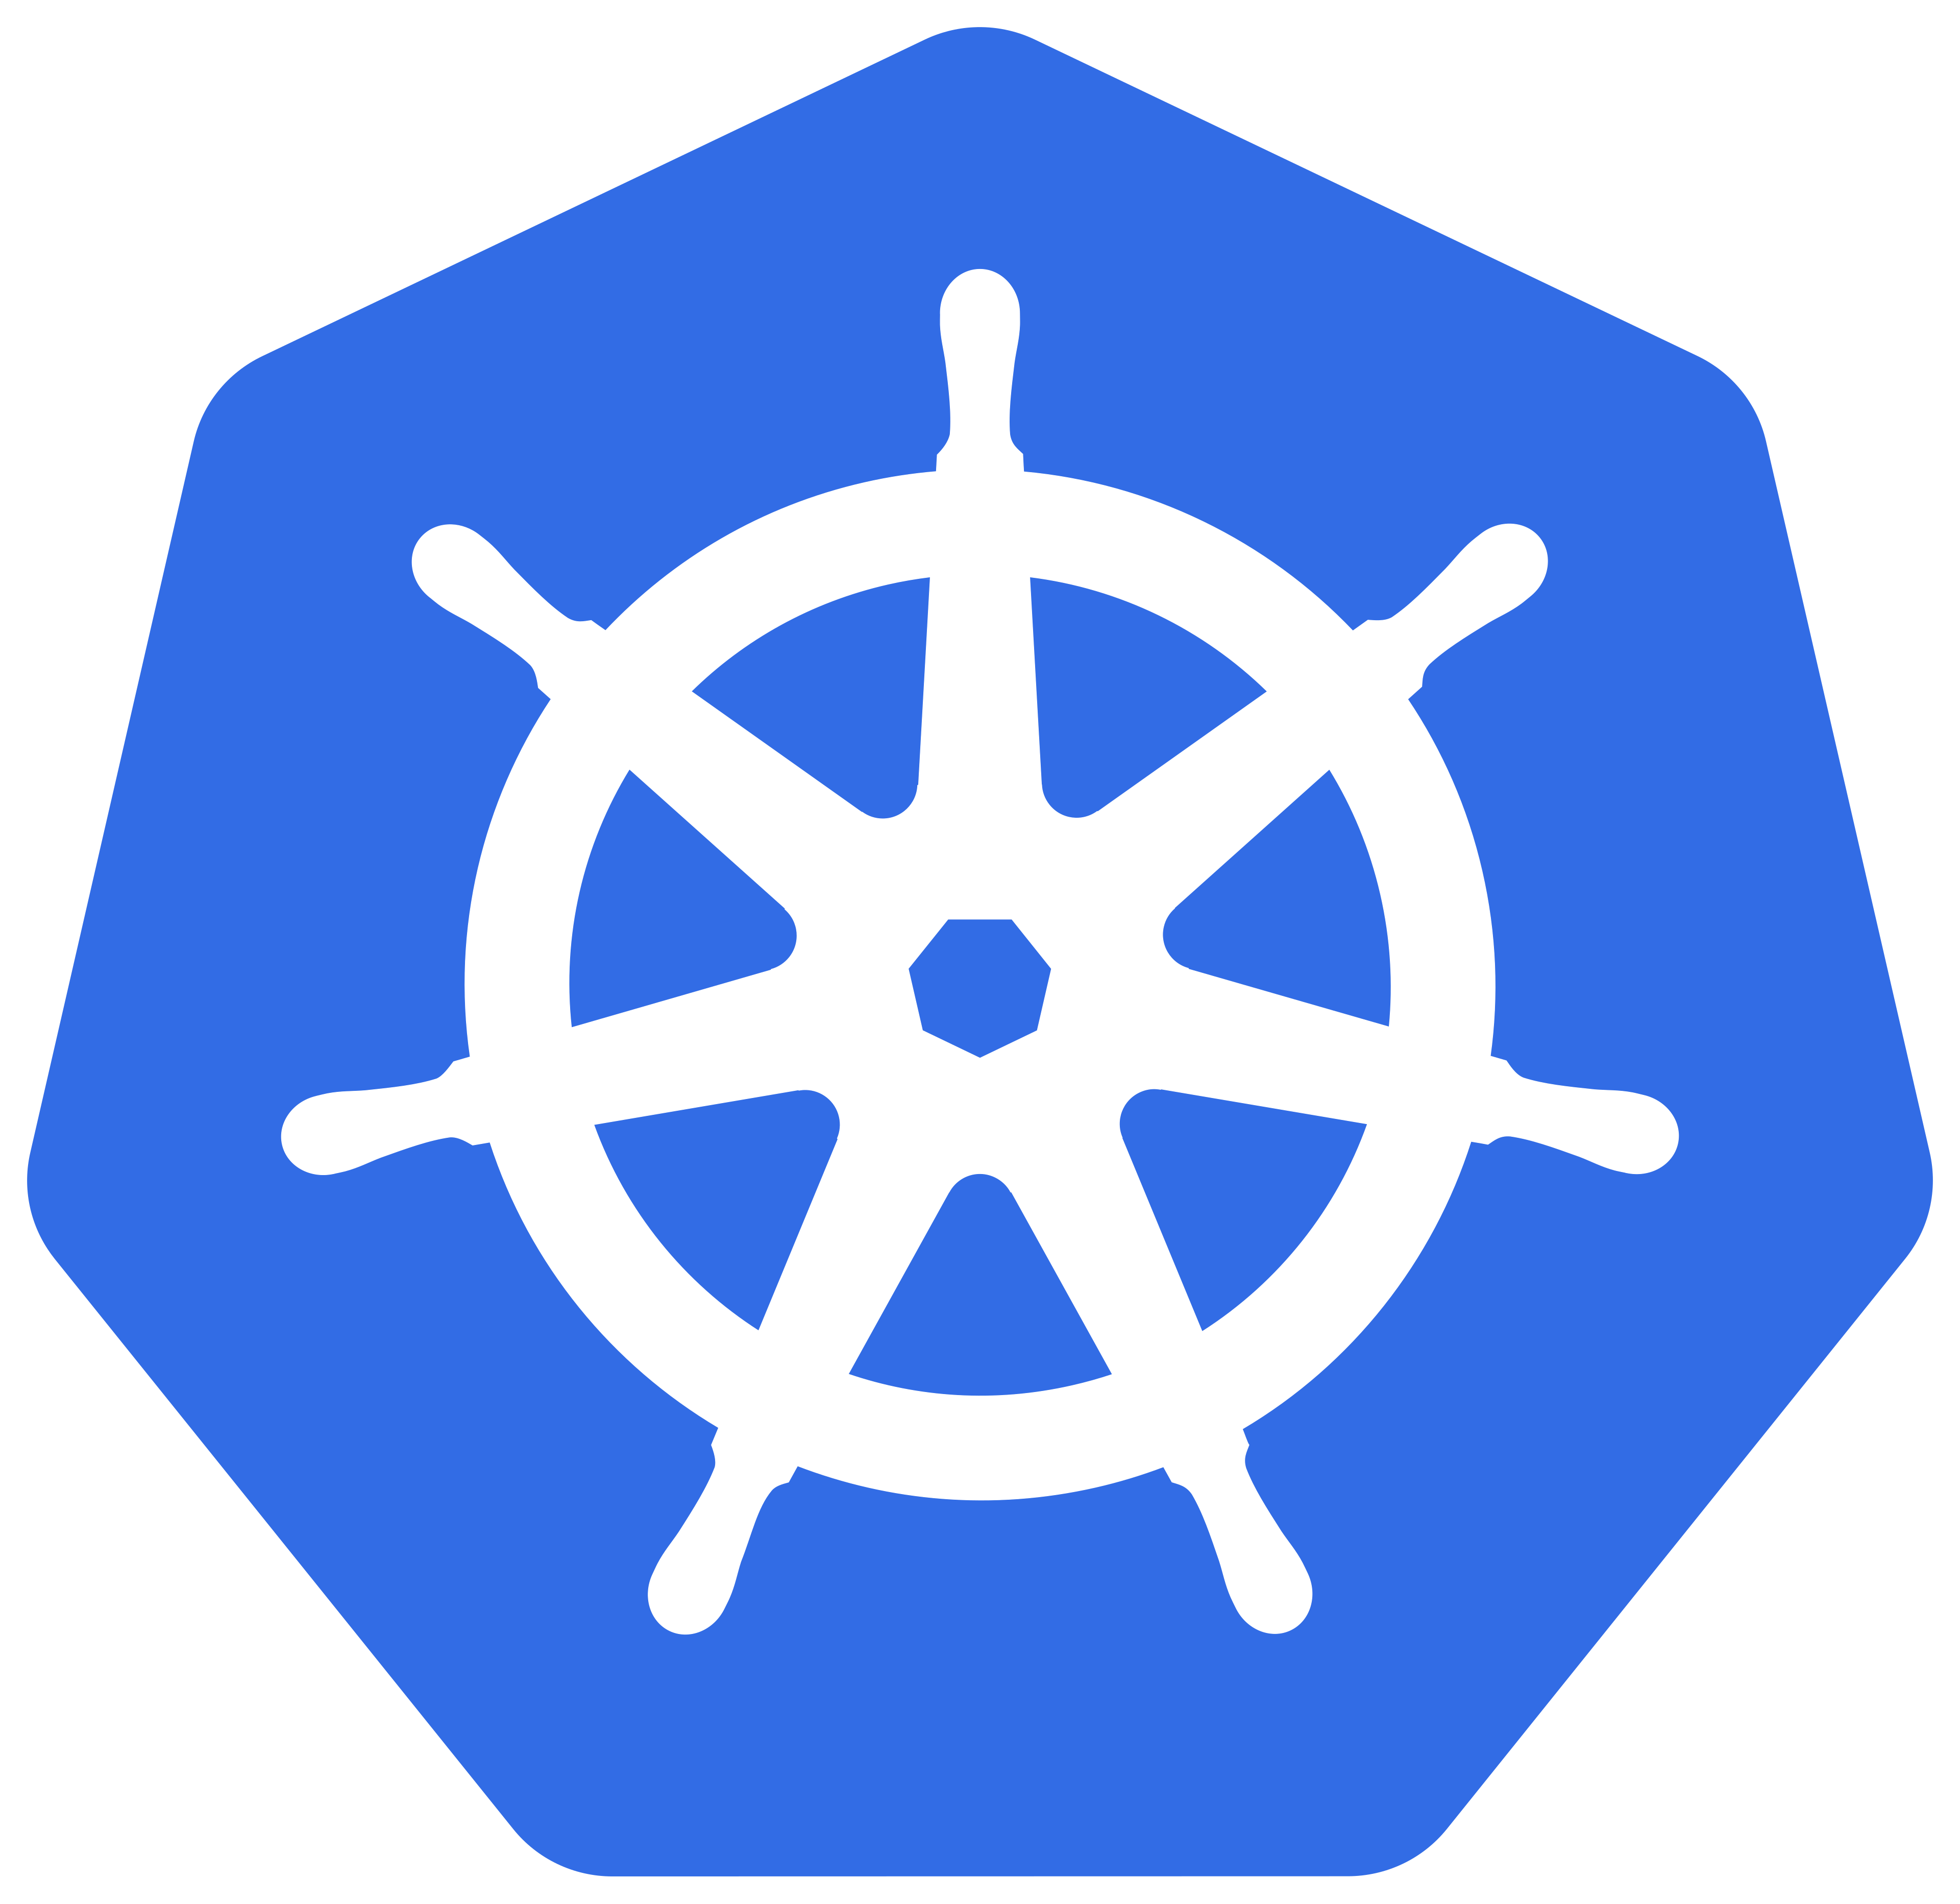
\includegraphics[height=0.48cm]{assets/kube-logo.png}\enspace
   {\sffamily\bfseries\small K3d / K3s}\quad
   {\sffamily\footnotesize namespace bnpb-m1; satu server, dua agen}};

\node[card] (host) at (1.25,5.45) {\textbf{Klien}\\host};
\node[service] (lb) at (4.65,5.45) {\textbf{K3d LB}\\serverlb};
\node[service] (api) at (7.75,5.45) {\textbf{Client API}\\NodePort 30080};

\node[service] (auth) at (7.75,3.55) {\textbf{Auth Service}\\ClusterIP};
\node[service] (agg) at (10.95,3.55) {\textbf{Aggregator}\\ClusterIP};
\node[service,minimum width=3.15cm] (sources) at (14.25,3.55)
  {\raisebox{-0.09cm}{
\includegraphics[height=0.38cm]{assets/bmkg-logo.png}}\enspace
   \raisebox{-0.08cm}{
\includegraphics[height=0.36cm]{assets/pvmbg-logo.png}}\\
   \textbf{BMKG / PVMBG}};

\node[state] (postgres) at (7.75,1.48) {\textbf{PostgreSQL}\\PVC 2 GiB};
\node[state] (rabbit) at (10.95,1.48)
  {\raisebox{-0.10cm}{
\includegraphics[height=0.39cm]{assets/rabbitmq-logo.png}}\enspace
   \textbf{RabbitMQ}\\PVC 1 GiB};
\node[service,minimum width=3.15cm] (consumers) at (14.25,1.48)
  {\textbf{Tiga konsumen}\\Deployment terpisah};

\draw[flow] (host.east) -- node[edgeword,above]{HTTP} (lb.west);
\draw[flow] (lb.east) -- (api.west);
\draw[flow] (api.south) -- (auth.north);
\draw[flow] (api.south east) -- (agg.north west);
\draw[flow] (auth.south) -- (postgres.north);
\draw[flow] (agg.south west) -- (postgres.north east);
\draw[flow] (agg.south) -- (rabbit.north);
\draw[flow] (agg.east) -- (sources.west);
\draw[flow] (rabbit.east) -- (consumers.west);
\end{tikzpicture}

\caption[Topologi uji lokal K3d/K3s]{\textbf{Klaster lokal memisahkan layanan dan penyimpanan persisten.} Client API diakses melalui NodePort 30080; layanan lain berkomunikasi pada jaringan internal. PostgreSQL berjalan sebagai StatefulSet satu replika dengan volume 2 GiB, dan RabbitMQ memakai PVC 1 GiB. Keduanya menjadi titik kegagalan tunggal pada konfigurasi ini.}
\label{fig:k3d}
\eraserlink{https://app.eraser.io/workspace/LNBH6Hy1uRmyFxbz4AFM?diagram=eCwmCAkSK__P3UMjd5Xo&layout=canvas}
\end{figure}

\section{Teknologi dan Alasan Pemilihan}

\subsection{Bahasa, kerangka kerja, dan batas transport}

Go digunakan pada mock sumber, Aggregator, Auth Service, Client API, consumer, dan Demo API. Dukungan konkurensi serta pustaka jaringan Go sesuai untuk layanan yang berkomunikasi melalui HTTP, gRPC, dan AMQP. Setiap layanan dibangun sebagai executable dan image container terpisah.

Gin hanya digunakan pada batas transport HTTP. Handler memproses request dan respons, sementara pemetaan data, otorisasi, dan use case berada pada lapisan aplikasi yang sesuai. Demo Console menggunakan React dan TypeScript; perannya terbatas pada pengujian dan demonstrasi.

\subsection{Protokol komunikasi}


\textbf{REST/JSON.} Aggregator mengambil data dari BMKG dan PVMBG melalui endpoint yang ditentukan spesifikasi. Tiap sumber mempertahankan identitas, autentikasi, dan bentuk responsnya; parameter waktu membatasi data sejak polling sebelumnya.


\textbf{gRPC/Protobuf.} Client API memanggil Auth Service dan Aggregator melalui kontrak pesan dan operasi internal yang eksplisit \cite{grpc-core}. Lapisan ini menjaga batas antarlayanan tanpa mengganti kontrak REST milik sumber.


\textbf{AMQP/RabbitMQ.} Exchange fanout menyalurkan satu event ke antrean tiap konsumen tanpa bergantung pada routing key \cite{rabbit-exchanges}. Konfirmasi penerbit membuktikan broker menerima pesan; pengakuan konsumen menandai pemrosesan berhasil \cite{rabbit-confirms}. Pesan yang ditolak tanpa pengantrean ulang diarahkan ke dead-letter exchange \cite{rabbit-dlx}.

\subsection{Penyimpanan}

PostgreSQL menyimpan data inti dalam kolom relasional dan atribut spesifik sumber dalam JSONB. JSONB mendukung operasi serta pengindeksan atas data terstruktur yang berubah \cite{postgres-jsonb}. Pada rancangan ini, JSONB menampung atribut tambahan, bukan menggantikan validasi data inti.

Akses PostgreSQL dibatasi pada layanan pemilik data. Aggregator menyimpan kejadian kanonik, sedangkan Auth Service menyimpan data autentikasi dengan kredensial terpisah. Pemisahan ini mempertahankan kepemilikan data meskipun layanan berbagi satu instance PostgreSQL pada deployment lokal.


\begin{table}[htbp]
\centering
\caption{\textbf{Pilihan teknologi mengutamakan batas layanan dan operasional prototipe.} Alternatif dicatat bersama konsekuensinya.}
\label{tab:tradeoffs}
\footnotesize
\begin{tabularx}{\textwidth}{L{2.25cm}L{4.0cm}Y}
\toprule
\textbf{Keputusan} & \textbf{Alternatif} & \textbf{Pilihan dan implikasi}\\
\midrule
Data dinamis & Kolom tetap, penyimpanan dokumen, atau JSONB. & \textbf{JSONB} mempertahankan kolom inti yang bertipe sekaligus menerima atribut aditif tanpa migrasi per field; validasi inti tetap dilakukan aplikasi.\\
\addlinespace[3pt]
RPC internal & REST/JSON atau gRPC/Protobuf. & \textbf{gRPC/Protobuf} memberi kontrak operasi internal yang eksplisit. REST/JSON tetap mengikuti kontrak sumber yang diwajibkan.\\
\addlinespace[3pt]
Distribusi event & Pemanggilan sinkron per konsumen atau broker pesan. & \textbf{RabbitMQ} menyediakan antrean terpisah; pengiriman setidaknya satu kali menuntut konsumen idempoten.\\
\addlinespace[3pt]
Deployment lokal & Proses gabungan atau kontainer per layanan. & \textbf{Kontainer dan K3d} memungkinkan pembangunan ulang layanan secara terpisah, dengan biaya orkestrasi yang lebih tinggi.\\
\bottomrule
\end{tabularx}
\end{table}

\subsection{Orkestrasi dan pengujian}

Docker Compose digunakan untuk menjalankan stack lokal. K3d menyediakan cluster K3s lokal, sedangkan Kustomize mengelola manifest dasar dan overlay. Pada Kubernetes, Service menyediakan jalur stabil menuju Pod; NodePort mengekspos service pada port tertentu di node \cite{kubernetes-service}. StatefulSet digunakan untuk PostgreSQL karena identitas Pod dan penyimpanan persisten dapat dikaitkan melalui volume claim template \cite{kubernetes-statefulset}.

Uji beban mengukur jumlah pengguna virtual, laju permintaan, durasi respons, persentil latensi, dan tingkat kesalahan. Ambang pengujian menetapkan batas lulus untuk latensi dan kegagalan permintaan \cite{k6-thresholds}. Hasil pada laporan ini menggambarkan konfigurasi lokal yang diuji, bukan jaminan kapasitas produksi.

\section{Asumsi dan Kebijakan Desain}

\subsection{Asumsi operasional}

BMKG dan PVMBG diperlakukan sebagai layanan otonom yang hanya merespons request. Aggregator melakukan polling dengan interval default 3 detik. Mock menyiapkan 20 record awal dan menghasilkan record baru dengan interval default 10 detik. Delay simulasi BMKG default 100 ms, sedangkan PVMBG memakai rentang 500 ms hingga 3 detik. Nilai tersebut adalah parameter eksperimen, bukan karakteristik layanan produksi.

Port, kredensial, interval, dan konfigurasi runtime dibaca dari environment. Secret aktual disediakan secara lokal atau melalui Kubernetes Secret dan tidak ditanam pada source code. Seluruh klien hilir bersifat hanya-baca pada M1.

\subsection{Kebijakan desain}


\textbf{Evolusi skema.} Atribut baru yang tidak termasuk field kanonik dipertahankan dalam JSONB. Perubahan nama, tipe, atau hilangnya field wajib memerlukan penanganan eksplisit; aplikasi tidak menebak makna kontrak sumber.


\textbf{Ketersediaan.} Gangguan satu sumber tidak menghentikan pembacaan data sumber lain. Data tersimpan tetap tersedia, tetapi statusnya ditandai usang agar pembaca tidak menafsirkannya sebagai pengamatan waktu nyata.


\textbf{Batas kepercayaan.} BMKG, PVMBG, layanan internal BNPB, dan klien hilir memakai identitas berbeda. Auth Service memvalidasi token dan cakupan akses; Client API membatasi proyeksi di sisi server. Token penyegaran disimpan sebagai hash dan dirotasi saat digunakan.


\textbf{Pengiriman event.} Outbox dan RabbitMQ menggunakan pengiriman setidaknya satu kali. Konsumen menekan pemrosesan ganda berdasarkan identitas kejadian selama proses berjalan. Karena catatan deduplikasi belum persisten, perlindungan itu tidak bertahan setelah konsumen dimulai ulang.

\subsection{Metode evaluasi}

\textbf{Lingkungan dan bukti.} Skenario ujung ke ujung P1--P5 dijalankan pada stack Docker Compose terisolasi pada 25 September 2026. Seluruh angka P1--P5 dalam makalah ini berasal dari satu run akhir yang sama. Pengamatan mencakup respons API, status sumber, identitas kontainer, isi basis data, panjang antrean, dan log dengan ID korelasi. Masa berlaku token diatur menjadi 60 detik agar kedaluwarsa dapat diamati tanpa memajukan jam.

\textbf{Pengukuran beban.} Dua run k6 pada 24 September 2026 mengukur pembacaan melalui Client API. Uji isolasi menggunakan 25 pengguna virtual per sumber selama 30 detik; uji berkelanjutan menggunakan 50 pengguna virtual selama 60 detik. Persentil latensi, laju permintaan, galat tak terduga, dan penolakan HTTP 429 diperoleh dari ringkasan mesin dan dilaporkan pada Tabel~\ref{tab:load-results}.

\textbf{Batas inferensi.} Semua sumber merupakan simulasi dan tiap skenario beban hanya memiliki satu run pada konfigurasi lokal. Hasilnya menilai perilaku prototipe yang diuji, bukan kapasitas produksi atau latensi layanan BMKG dan PVMBG yang sebenarnya.

\section{Problem 1: Arsitektur dan Interoperabilitas Data}

\subsection{Rancangan solusi}

\textbf{Pemetaan sumber.} Aggregator membentuk HazardEvent dari identitas, lokasi, waktu, dan keparahan kejadian. Peringatan tsunami BMKG dikaitkan melalui identitas gempa; laporan PVMBG memperoleh nama area dan koordinat dari tabel referensi gunung api. Rincian seperti magnitudo, tinggi kolom abu, dan tingkat keyakinan tetap disimpan dalam atribut JSONB \cite{postgres-jsonb}.

\textbf{Aturan keparahan.} Tanpa tingkat ancaman tsunami yang dikenali, keparahan gempa ditentukan oleh magnitudo $m$:
\begin{equation}
s_m(m)=
\begin{cases}
\text{normal}, & m<5{,}0,\\
\text{waspada}, & 5{,}0\le m<6{,}5,\\
\text{siaga}, & m\ge6{,}5.
\end{cases}
\label{eq:severity}
\end{equation}
Tingkat ancaman \emph{waspada}, \emph{siaga}, atau \emph{awas} pada peringatan yang terkait menggantikan hasil Persamaan~\ref{eq:severity}; nilai ancaman lain kembali ke aturan magnitudo. Tingkat aktivitas PVMBG dipetakan langsung ke kategori keparahan yang sama.

\subsection{Penanganan perubahan skema}

Field wajib yang dibaca dari payload diperiksa jenis dan keberadaannya, sedangkan atribut tambahan dipertahankan tanpa mengubah tabel kanonik. Penambahan \code{confidence_level} karena itu tidak memerlukan migrasi per atribut. Pemeriksaan bahwa \code{volcano_id} benar-benar ada dalam tabel referensi belum eksplisit pada pemetaan PVMBG; validasi lokasi tidak diklaim untuk ID yang tidak dikenal.

\subsection{Konsekuensi pilihan dan batasan}

Pemetaan dinamis mengurangi coupling pada daftar field sumber, sedangkan field kanonik mempertahankan tipe dan konsistensi yang dibutuhkan query. JSONB tidak menghilangkan kebutuhan validasi aplikasi. Perubahan semantik, rename, perubahan tipe, dan penghilangan field wajib tidak dianggap perubahan aditif; semuanya membutuhkan perubahan kontrak atau kode yang eksplisit. Query atas atribut dinamis juga memerlukan aturan aplikasi yang jelas.

\subsection{Pengujian dan bukti}

\textbf{Penambahan atribut tidak memerlukan migrasi tabel pada run lokal.} Snapshot akhir run E2E menunjukkan 90 HazardEvent BMKG dan 90 PVMBG. Sebanyak 25 record PVMBG tanpa \code{confidence_level} dan 65 record dengannya dapat dibaca bersama setelah perubahan saat layanan berjalan. Hasil ini membuktikan kompatibilitas penambahan atribut pada data uji; perubahan nama atau tipe field tidak diuji.

\begin{evidencebox}{Observasi pemetaan dan evolusi skema}
\begin{lstlisting}
canonical events: BMKG=90; PVMBG=90
PVMBG before update: 25 records without confidence_level
PVMBG after update: 65 records with confidence_level
runtime update: Aggregator and PVMBG container IDs unchanged

BMKG sample: SOURCE_BMKG / HAZARD_TYPE_SEISMIC / SEVERITY_WASPADA
  attributes: magnitude=5.1, depth_km=12, potential_tsunami=true
PVMBG sample: SOURCE_PVMBG / HAZARD_TYPE_VOLCANIC / SEVERITY_WASPADA
  attributes: eruption_count_24h=1, ash_column_height_m=350
PVMBG after update: attributes.confidence_level=0.82
\end{lstlisting}
\end{evidencebox}

\section{Problem 2: Konkurensi, Ketersediaan, dan Degradasi}

\subsection{Rancangan solusi}

Aggregator menjalankan polling BMKG dan PVMBG secara independen. Batas waktu mencegah panggilan keluar menunggu tanpa akhir; kegagalan satu siklus tidak membatalkan siklus sumber lain. Client API membatasi jumlah permintaan serentak dan lamanya pemrosesan untuk mengendalikan pemakaian sumber daya.

Jika polling PVMBG gagal, Aggregator mempertahankan data terakhir dan menandai sumber sebagai usang. Data BMKG tetap dapat dibaca. Setelah gangguan berakhir, status PVMBG kembali normal pada siklus polling berikutnya tanpa memulai ulang layanan.

\subsection{Metode dan hasil uji beban}

Uji isolasi menjalankan 25 pengguna virtual untuk pembacaan BMKG dan 25 untuk PVMBG selama 30 detik, sementara batas penundaan polling PVMBG dikonfigurasi hingga 3 detik. k6 mengukur waktu respons baca Client API, bukan panggilan langsung ke sumber. Dari 27.558 permintaan, laju gabungan tercatat 914,981 permintaan per detik. Pembacaan BMKG menghasilkan p50 3,445 ms, p95 8,790 ms, dan p99 19,462 ms; p95 pembacaan PVMBG sebesar 8,425 ms. \textbf{p95 pembacaan BMKG berada di bawah ambang 300 ms} pada run ini, tanpa galat maupun penolakan kapasitas.

Uji berkelanjutan memakai 50 pengguna virtual selama 60 detik untuk pembacaan data BMKG. Run menghasilkan 28.211 permintaan dengan laju 468,899 permintaan per detik. Latensi p50, p95, dan p99 masing-masing 4,888 ms, 13,970 ms, dan 19,915 ms. Tingkat kesalahan dan penolakan kapasitas terkontrol tercatat 0\%. Ambang evaluasi mengukur persentil latensi serta proporsi permintaan gagal \cite{k6-thresholds}.

\begin{table}[htbp]
\centering
\caption[Hasil dua skenario uji beban lokal]{\textbf{Pembacaan BMKG memenuhi ambang p95 pada dua skenario lokal.} Angka berasal dari run k6 pada 24 September 2026 melalui Client API.}
\label{tab:load-results}
\footnotesize
\setlength{\tabcolsep}{3.5pt}
\begin{tabularx}{\textwidth}{L{2.1cm}Y R{1.55cm}R{1.4cm}R{1.0cm}R{1.0cm}R{1.0cm}R{1.0cm}}
\toprule
\textbf{Skenario} & \textbf{Beban/durasi} & \textbf{Permintaan} & \textbf{Laju (req/s)} & \textbf{p50 (ms)} & \textbf{p95 (ms)} & \textbf{p99 (ms)} & \textbf{Galat}\\
\midrule
Isolasi sumber & 25 VU per sumber; 30 s & 27.558 & 914,981 & 3,445 & \cellcolor{metablue!10}\textbf{8,790} & 19,462 & 0\%\\
Berkelanjutan & 50 VU; 60 s & 28.211 & 468,899 & 4,888 & 13,970 & 19,915 & 0\%\\
\bottomrule
\end{tabularx}
\par\vspace{2pt}{\footnotesize\raggedright Catatan: pada baris isolasi, jumlah permintaan dan laju menggabungkan dua sumber; persentil latensi hanya untuk endpoint baca BMKG. VU = pengguna virtual.\par}
\end{table}

\begin{figure}[htbp]
\centering
\begin{minipage}[c]{0.66\linewidth}
\begin{tikzpicture}
\begin{axis}[
  width=\linewidth,
  height=5.0cm,
  xmin=0.55,xmax=3.45,
  xtick={1,2,3},
  xticklabels={p50,p95,p99},
  ymin=0,
  ymax=23,
  ytick={0,5,10,15,20},
  xlabel={Persentil latensi},
  ylabel={Latensi (ms)},
  ymajorgrids=true,
  xmajorgrids=false,
  axis lines*=left,
  axis line style={draw=metafg!65,line width=0.55pt},
  tick label style={font=\footnotesize},
  label style={font=\footnotesize},
  clip=false,
]
\addplot+[only marks,mark=*,mark size=2.6pt,mark options={fill=metablue,draw=metablue}] coordinates {
  (0.88,3.445) (1.88,8.7898) (2.88,19.46156)
};
\addplot+[only marks,mark=square*,mark size=2.5pt,mark options={fill=metafg!70,draw=metafg!70}] coordinates {
  (1.12,4.888) (2.12,13.970) (3.12,19.91538)
};
\end{axis}
\end{tikzpicture}
\end{minipage}\hfill
\begin{minipage}[c]{0.30\linewidth}
\begin{tcolorbox}[
  colback=metabg,frame hidden,
  borderline west={2pt}{0pt}{metablue},
  arc=2mm,
  left=3mm,right=2.5mm,top=2.5mm,bottom=2.5mm
]
{\footnotesize\sffamily\bfseries\color{metafg}HASIL UTAMA}\par\smallskip
{\Large\sffamily\bfseries\color{metablue}8,79 ms}\par
{\small p95 baca BMKG, uji isolasi}\par\medskip
{\small\textbf{Ambang} 300 ms\\
\textbf{Rasio} 2,9\% dari ambang}
\end{tcolorbox}
\vspace{0.5em}
{\footnotesize
\tikz\fill[metablue] (0,0) circle (2pt);\ Isolasi BMKG\\
\tikz\fill[metafg!70] (0,0) rectangle (4pt,4pt);\ Beban BMKG
}
\end{minipage}
\caption[Persentil latensi pembacaan BMKG]{\textbf{p95 pembacaan BMKG berada di bawah ambang pada dua run lokal.} Seri biru menunjukkan uji isolasi 25 pengguna virtual per sumber selama 30 detik saat polling PVMBG diberi penundaan hingga 3 detik; seri gelap menunjukkan uji berkelanjutan 50 pengguna virtual selama 60 detik. Latensi diukur melalui Client API pada 24 September 2026. Ambang 300 ms ditampilkan terpisah karena di luar skala grafik.}
\label{fig:load-percentiles}
\end{figure}

\textbf{Gangguan hanya mengubah kesegaran PVMBG.} Pembacaan BMKG dan data PVMBG yang telah tersimpan tetap berhasil ketika sumber vulkanik tidak tersedia. Setelah gangguan berakhir, status PVMBG pulih tanpa memulai ulang layanan.

\subsection{Konsekuensi pilihan, batasan, dan bukti}

Data terakhir mempertahankan sebagian fungsi baca ketika PVMBG tidak tersedia, tetapi memiliki risiko kebaruan. Karena itu status stale harus ikut diperiksa. Timeout dan batas inflight mengendalikan konsumsi resource, tetapi dapat membatasi throughput atau menghasilkan HTTP 429 saat kapasitas tercapai. Angka k6 merepresentasikan satu konfigurasi run lokal; angka tersebut bukan SLA produksi dan tidak membandingkan variasi spesifikasi host.


\begin{evidencebox}{Keluaran pengukuran dan observasi outage}
\begin{lstlisting}
load run (24 Sep 2026): VU=50; duration=60.16 s; requests=28211
throughput=468.899 req/s; p50=4.888 ms; p95=13.970 ms; p99=19.915 ms
error_rate=0%; controlled_rejections=0
outage: PVMBG healthy -> stale (stale_since set)
requests during outage: BMKG=HTTP 200; PVMBG stored data=HTTP 200
recovery: PVMBG healthy; no service restart
\end{lstlisting}
\end{evidencebox}

\section{Problem 3: Autentikasi Antarlayanan dan Batas Kepercayaan}

\subsection{Pemisahan domain kredensial}

Setiap sumber, layanan internal, dan klien hilir memiliki identitas tersendiri. BMKG memvalidasi kunci akses khusus sumber, sedangkan PVMBG memvalidasi token pembawa. Komunikasi internal memakai kredensial layanan tersendiri. Auth Service mengelola akses Media, Tim Lapangan, dan BNPB Ops.

\begin{table}[htbp]
\centering
\caption{\textbf{Kredensial tiap domain divalidasi oleh layanan pemiliknya.} Cakupan akses klien diterapkan kembali pada Client API.}
\label{tab:trust-domains}
\small
\begin{tabularx}{\textwidth}{L{3.2cm}L{5.0cm}Y}
\toprule
\textbf{Domain} & \textbf{Kredensial} & \textbf{Pemilik validasi}\\
\midrule
BMKG & Kunci akses khusus BMKG & Simulasi BMKG\\
PVMBG & Token akses khusus PVMBG & Simulasi PVMBG\\
\addlinespace[2pt]
Internal BNPB & Kredensial antarlayanan & Layanan internal terkait\\
\addlinespace[2pt]
Media & Kredensial berhak ringkasan & Auth Service\\
Tim Lapangan & Kredensial berhak data lapangan & Auth Service\\
BNPB Ops & Kredensial berhak data lengkap & Auth Service\\
\bottomrule
\end{tabularx}
\end{table}

\subsection{Cakupan akses, token, dan proyeksi}

Auth Service menerbitkan token dengan cakupan akses sesuai identitas. Media hanya memperoleh ringkasan, sedangkan Tim Lapangan dan BNPB Ops dapat memperoleh data mentah sesuai perannya. Client API memvalidasi token dan menegakkan cakupan tersebut di sisi server. Permintaan data mentah dari Media ditolak dengan HTTP 403; pembatasan tidak hanya bergantung pada tampilan antarmuka.

Access token berlaku selama 60 detik pada konfigurasi pengujian. Refresh token disimpan dalam bentuk hash dan dirotasi ketika digunakan. Token lama setelah rotasi ditolak. Masa berlaku diuji secara alami, bukan dengan memajukan jam sistem.

\subsection{Konsekuensi pilihan, batasan, dan pengujian}

Pemisahan trust mencegah penggunaan kredensial satu sumber pada sumber lain dan menempatkan enforcement data mentah di server. Auth Service menambahkan satu panggilan gRPC pada validasi akses, tetapi memusatkan penerbitan, validasi, dan rotasi token. M1 belum mengintegrasikan identity provider eksternal atau revocation list terdistribusi.

\textbf{Penolakan akses diterapkan pada batas layanan.} Kredensial silang BMKG dan PVMBG menghasilkan HTTP 401. Media mendapat HTTP 403 untuk data mentah, tetapi dapat membaca ringkasan tanpa koordinat dan atribut sumber; BNPB Ops dapat membaca data mentah. Token akses kedaluwarsa setelah 60 detik, sedangkan penggunaan ulang token penyegaran yang sudah dirotasi ditolak. Pemindaian konfigurasi tidak menemukan kandidat kredensial tertanam, dengan batas bahwa pemeriksaan tersebut bersifat heuristik.

\begin{evidencebox}{Ringkasan audit konfigurasi}
\begin{lstlisting}
configuration template tracked: yes
other tracked environment files: 0
credential-signature candidates in tracked code/configuration: 0
scan: high-confidence private-key and provider-token patterns plus long literal assignments
\end{lstlisting}
\noindent\small Pemindaian bersifat heuristik dan tidak menjamin deteksi semua format rahasia; tidak ada nilai kredensial yang disimpan dalam bukti.
\end{evidencebox}

\begin{evidencebox}{Urutan respons akses yang diamati}
\begin{lstlisting}
credential silang BMKG/PVMBG: HTTP 401 / HTTP 401
Media meminta data mentah: HTTP 403
Media membaca ringkasan: HTTP 200; koordinat dan attributes tidak ada
BNPB Ops membaca data mentah: HTTP 200; field mentah tersedia
Field Team setelah TTL 60 s: HTTP 401
refresh token: HTTP 200; penggunaan ulang refresh token lama: HTTP 401
\end{lstlisting}
\noindent\small Keluaran E2E mencatat kode respons dan hasil proyeksi; nilai secret serta token tidak disimpan dalam bukti.
\end{evidencebox}

\section{Problem 4: Batas Layanan dan Penyimpanan Fleksibel}

\subsection{Batas layanan}

BMKG dan PVMBG merupakan mock source independen. Aggregator menangani polling, pemetaan, status sumber, Canonical Store, dan outbox. Auth Service mengelola client serta token. Client API menyajikan endpoint downstream dan menegakkan otorisasi. Dashboard, Notifier, dan Portal merupakan consumer terpisah. Batas ini memungkinkan salah satu layanan dibangun ulang tanpa mengemas ulang seluruh sistem.

\subsection{Penyimpanan dan kepemilikan data}

PostgreSQL menyimpan HazardEvent pada kolom kanonik serta atribut fleksibel dalam JSONB. Dalam deployment lokal, satu instance PostgreSQL menyediakan penyimpanan terpisah bagi Aggregator dan Auth Service dengan peran akses berbeda. Aggregator menjadi pemilik Canonical Store. Tugas migrasi satu kali menggunakan kredensial milik Aggregator untuk menyiapkan skema; layanan runtime lain tidak menerima URL tersebut. Peran Auth tidak memiliki hak SELECT pada tabel HazardEvent, sementara Client API membaca data melalui API Aggregator dan consumer menerima event melalui broker. Sarana demonstrasi tidak memiliki akses database maupun kendali terhadap container.

\subsection{Alternatif dan pertukaran}

Skema relasional tetap memudahkan tipe dan query tetapi setiap field baru dapat memerlukan migrasi. Document store fleksibel terhadap bentuk dokumen, namun menambah teknologi dan pola query baru. JSONB dipilih sebagai kompromi: field inti tetap relasional, atribut tambahan dapat berdampingan, dan penambahan field sumber tidak menuntut perubahan tabel. Konsekuensinya, aplikasi tetap bertanggung jawab memvalidasi field kanonik dan membatasi query atribut dinamis.

\subsection{Penerapan dan pengujian}

Pada K3d, workload memiliki satu replika secara default. PostgreSQL berjalan sebagai StatefulSet satu replika dengan volume claim template 2 GiB. RabbitMQ berjalan satu replika dengan PVC 1 GiB. Overlay lokal mengekspos Client API melalui NodePort 30080; port host dipetakan ke load balancer K3d. Tidak ada Ingress pada overlay lokal. Service NodePort menerima trafik pada port node dan meneruskannya ke Service/endpoint terkait \cite{kubernetes-service}; StatefulSet mempertahankan identitas Pod dan storage terkait \cite{kubernetes-statefulset}.

\textbf{Pembangunan ulang PVMBG tidak mengubah Aggregator maupun Client API.} Identitas kedua kontainer tetap sama dan pembacaan BMKG masih menghasilkan HTTP 200. Pemeriksaan konfigurasi menunjukkan hanya Aggregator dan tugas migrasinya menerima URL Canonical Store; peran Auth tidak memiliki hak SELECT pada HazardEvent. Sebanyak 25 record lama dan 65 record baru tetap terbaca tanpa perubahan struktur tabel.

\begin{evidencebox}{Observasi rebuild dan kepemilikan penyimpanan}
\begin{lstlisting}
PVMBG container: b35925c4cddd -> 86cecb7978f8 (rebuilt)
Aggregator container: a041fba24f5c -> a041fba24f5c (unchanged)
Client API container: 571b6e639d1a -> 571b6e639d1a (unchanged)
BMKG query after PVMBG rebuild: HTTP 200
canonical database URL: Aggregator=yes; one-shot migrator=yes
runtime services (API, Auth, sources, consumers): no canonical URL
Auth database role SELECT on hazard_events: denied
old/new PVMBG records without/with confidence_level: 25/65
\end{lstlisting}
\noindent\small Pemeriksaan menunjukkan bahwa tugas migrasi memakai kredensial pemilik store, sedangkan layanan runtime lain tidak menerimanya. Hak SELECT peran Auth juga diperiksa pada PostgreSQL; kebijakan firewall jaringan tidak menjadi bagian dari probe ini.
\end{evidencebox}

\section{Problem 5: Distribusi Event kepada Banyak Konsumen}

\subsection{Produsen, broker, dan konsumen}

Aggregator menyimpan HazardEvent dan pesan outbox dalam satu transaksi. Outbox worker menerbitkan pesan persisten ke exchange fanout RabbitMQ, yang menyalurkan salinan event ke antrean durable tiap konsumen \cite{rabbit-exchanges}. Producer tidak memanggil konsumen secara sinkron.

Publisher menunggu konfirmasi penerimaan broker, sedangkan konsumen mengakui pesan setelah pemrosesan berhasil. Pesan yang terus gagal dapat dipisahkan dari antrean utama melalui mekanisme dead-letter. Konfirmasi publisher dan acknowledgement konsumen melindungi dua sisi pengiriman yang berbeda \cite{rabbit-confirms}.

\subsection{Semantik pengiriman dan idempotensi}

Outbox serta broker menggunakan pengiriman setidaknya satu kali; pesan dapat diterima ulang bila hasil publikasi atau pemrosesan tidak dapat dipastikan. Konsumen menekan pemrosesan ganda selama proses yang sama, tetapi catatan deduplikasi tidak bertahan setelah layanan dimulai ulang. Dengan demikian, sistem belum menjamin pemrosesan tepat satu kali secara persisten.

\subsection{Konsekuensi pilihan, batasan, dan pengujian}

RabbitMQ dipilih karena exchange fanout dan queue terpisah sesuai dengan kebutuhan M1 untuk mengisolasi consumer dan menambahkan subscriber tanpa perubahan producer. Kafka dapat menyediakan replay dan model log berpartisi, tetapi menambah kompleksitas operasional di luar kebutuhan demonstrasi lokal. Dead-lettering membantu memisahkan pesan yang ditolak, tetapi keberhasilan pemindahan dead-letter tetap bergantung pada konfigurasi broker \cite{rabbit-dlx}.

\textbf{Gangguan konsumen dan broker menghasilkan backlog yang pulih.} Saat Notifier berhenti, antreannya berubah dari 0 menjadi 8 pesan sementara Dashboard tetap menerima event; setelah Notifier aktif kembali, antrean menjadi nol dan event yang sama ditemukan pada lognya. Portal ditambahkan tanpa mengubah image producer. Saat broker berhenti, 10 pesan outbox tertunda lalu habis diterbitkan setelah broker pulih. Log ketiga konsumen memuat ID kejadian dan ID korelasi yang sama. Run ini tidak memaksakan pengiriman ulang, sehingga tidak membuktikan deduplikasi persisten.

\begin{evidencebox}{Log consumer dan pemulihan pesan}
\begin{lstlisting}
dashboard-consumer | event_id=ece5a4df | correlation_id=ee1bacfe | redelivered=false
notifier-consumer  | event_id=ece5a4df | correlation_id=ee1bacfe | redelivered=false
portal-consumer    | event_id=ece5a4df | correlation_id=ee1bacfe | redelivered=false
catch-up during stop/restart: event_id=3db89de1; correlation_id=4325cd2e
Notifier queue: 0 -> 8 -> 0; outbox while broker was down: 10 -> 0
\end{lstlisting}
\noindent\small ID pada cuplikan ditampilkan dengan delapan karakter pertama; pencocokan terhadap log lengkap memastikan kesamaan nilai. Selama Notifier berhenti, antreannya bertambah dari 0 menjadi 8, lalu kembali ke 0 setelah pemulihan. Sampel fan-out menunjukkan pengiriman normal; skenario ini tidak memaksakan redelivery.
\end{evidencebox}

\section{Observabilitas, Keamanan, dan Operasi}

\subsection{Pemeriksaan kesehatan dan pencatatan}

Layanan menyediakan pemeriksaan kesehatan untuk pemantauan pada container lokal maupun cluster Kubernetes. Aggregator juga melaporkan kesegaran BMKG dan PVMBG secara terpisah. Log terstruktur memuat nama layanan, operasi, hasil, latensi, dan ID korelasi sehingga alur permintaan lintas layanan dapat ditelusuri.

\subsection{Keamanan konfigurasi}

Kredensial aktual tidak ditanam pada kode aplikasi, image layanan, atau konfigurasi deployment. Berkas contoh hanya menjelaskan jenis konfigurasi yang diperlukan; nilai rahasia disediakan secara lokal atau melalui Secret Kubernetes. Layanan dijalankan dengan hak akses minimum. Auth Service memisahkan kredensial klien dan menyimpan token dalam bentuk hash; akses data mentah diperiksa di sisi server.

\subsection{Petunjuk menjalankan sistem}

Operasi lokal dimulai dengan menyediakan kredensial melalui mekanisme yang aman, menyiapkan kontrak komunikasi, lalu menjalankan layanan sebagai container terpisah. Setelah pemeriksaan kesehatan menyatakan layanan siap, pengujian fungsional dan skenario E2E digunakan untuk memvalidasi perilaku sistem.

Pada mode lokal, Docker Compose menjalankan layanan sumber, layanan koordinasi, basis data, dan broker dalam kontainer terpisah. Kontrak komunikasi disiapkan sebelum layanan dijalankan.

Setelah layanan siap, pemeriksaan kesehatan, uji unit, validasi kontrak, dan skenario E2E digunakan untuk menilai kesiapan dan perilaku sistem.

Untuk evaluasi klaster lokal, K3d menjalankan satu server dan dua agen. Akses klien masuk melalui NodePort, sementara komunikasi internal menggunakan Service Kubernetes. Layanan tanpa status dapat direplikasi; basis data dan broker tetap satu replika pada konfigurasi M1 sehingga keduanya menjadi titik kegagalan tunggal.

\section{Sintesis Hasil}

\subsection{Ringkasan hasil}

\begin{table}[htbp]
\centering
\caption{\textbf{Lima kriteria M1 teramati pada pengujian lokal.} Setiap hasil ditafsirkan dalam batas lingkungan simulasi dan satu run yang dilaporkan.}
\label{tab:test-summary}
\footnotesize
\begin{tabularx}{\textwidth}{L{1.25cm}L{3.4cm}YL{3.2cm}}
\toprule
\textbf{Masalah} & \textbf{Metode} & \textbf{Observasi utama} & \textbf{Batas inferensi}\\
\midrule
P1 & Evolusi skema saat layanan berjalan & \textbf{90 kejadian per sumber}; 25 record lama dan 65 baru tetap terbaca. & Hanya penambahan atribut yang diuji.\\
\addlinespace[3pt]
P2 & k6 isolasi dan beban berkelanjutan & \textbf{p95 baca BMKG 8,79 ms} pada isolasi; 28.211 permintaan dan galat 0\% pada 50 pengguna virtual. & Pembacaan melalui Client API pada stack lokal.\\
\addlinespace[3pt]
P3 & Kredensial silang dan hak data mentah & \textbf{HTTP 401} untuk kredensial silang; \textbf{HTTP 403} untuk akses mentah Media; token berakhir setelah 60 detik. & Identitas berasal dari layanan simulasi.\\
\addlinespace[3pt]
P4 & Pembangunan ulang PVMBG dan pemeriksaan hak basis data & \textbf{Aggregator dan Client API tetap berjalan}; peran Auth tidak dapat membaca HazardEvent. & Instance PostgreSQL masih dipakai bersama.\\
\addlinespace[3pt]
P5 & Penghentian Notifier dan broker lalu pemulihan & \textbf{Antrean 0--8--0}; outbox 10--0 pesan setelah pemulihan. & Pengiriman ulang tidak dipaksakan; deduplikasi belum persisten.\\
\bottomrule
\end{tabularx}
\end{table}

Gambar~\ref{fig:load-percentiles} memperlihatkan seluruh persentil pembacaan BMKG yang dilaporkan k6. Pada uji isolasi, p95 sebesar 8,790 ms setara dengan 2,9\% dari ambang 300 ms; pada uji berkelanjutan, p95 sebesar 13,970 ms. Kedua angka berasal dari satu run per skenario dan tidak menunjukkan variasi antarrun. Ambang galat di bawah 1\% juga terpenuhi pada run tersebut \cite{k6-thresholds}.

Rincian hubungan antara kriteria, pengamatan, dan batas interpretasi disajikan pada Tabel~\ref{tab:traceability} di Lampiran~\ref{sec:traceability}.

\subsection{Batasan evaluasi dan informasi yang perlu dilengkapi}

Skenario E2E P1--P5 dijalankan pada 25 September 2026 di dalam stack sementara yang dibersihkan setelah pengujian. Data uji beban berasal dari 24 September. Uji integrasi terpisah terhadap stack lokal tidak dijalankan; hasil E2E tidak disamakan dengan pengujian integrasi yang lebih luas. Angka beban tidak digunakan untuk menyimpulkan kapasitas produksi, dan deduplikasi konsumen belum persisten setelah restart. Integrasi API produksi BMKG/PVMBG tidak termasuk cakupan.

Nama kelompok tercatat sebagai SidequestProxy; pembagian kontribusi perlu dikonfirmasi oleh kelompok. Bukti disajikan melalui cuplikan log, hasil pengukuran, diagram, dan grafik; pembahasan menafsirkan hasil tanpa menyalin detail internal implementasi.

\section{Pernyataan Penggunaan LLM}

LLM digunakan sebagai alat bantu untuk menelusuri struktur repository, menyusun draft dokumentasi, merangkum hasil pengujian, dan membantu penyuntingan bahasa. Penggunaan tersebut tidak menggantikan tanggung jawab kelompok untuk memahami desain, memeriksa implementasi, dan memverifikasi bukti yang disajikan.

Sebelum laporan dikumpulkan, seluruh anggota kelompok perlu meninjau kode, konfigurasi, angka pengujian, dan naskah final. Klaim yang tidak dapat ditelusuri ke kode, dokumentasi, atau artefak run harus dihapus atau diperbaiki. Penggunaan LLM dinyatakan secara eksplisit sesuai ketentuan spesifikasi M1 \cite{spec-m1}.

\section{Kesimpulan}

Prototipe M1 mengintegrasikan dua layanan sumber simulasi melalui Aggregator, menyajikan HazardEvent kanonik kepada klien yang berwenang, dan mendistribusikan event melalui outbox serta RabbitMQ. Pemisahan kolom kanonik dan JSONB memungkinkan atribut tambahan PVMBG diterima tanpa migrasi per atribut, sementara akses langsung ke Canonical Store tetap dimiliki Aggregator.

Pada pengujian lokal, perubahan atribut aditif, gangguan sumber, penolakan akses tidak sah, pembangunan ulang layanan, dan pemulihan backlog menunjukkan perilaku yang sesuai dengan lima kriteria M1. Pembacaan BMKG melalui Client API memiliki p95 8,790 ms pada uji isolasi dengan batas penundaan polling PVMBG 3 detik, lebih rendah daripada ambang 300 ms. Angka ini menggambarkan satu konfigurasi prototipe dan tidak mengukur latensi sumber secara langsung. Pengiriman pesan tetap bersemantik setidaknya satu kali, sedangkan deduplikasi konsumen belum persisten setelah proses dimulai ulang. Kontribusi setiap anggota masih menunggu konfirmasi kelompok.

\begin{thebibliography}{99}
\bibitem[Tim Pengajar IF4031(2026)]{spec-m1}
Tim Pengajar IF4031. 2026.
\textit{Tugas Besar IF4031, Milestone 1: Sistem Terdistribusi Dasar}.
Dokumen spesifikasi tugas mata kuliah.

\bibitem[PostgreSQL Global Development Group(2026)]{postgres-jsonb}
PostgreSQL Global Development Group. 2026.
\textit{JSON Types}.
PostgreSQL 17 Documentation.
\url{https://www.postgresql.org/docs/17/datatype-json.html}.
Diakses 25 September 2026.

\bibitem[gRPC Authors(2026)]{grpc-core}
gRPC Authors. 2026.
\textit{Core concepts, architecture and lifecycle}.
\url{https://grpc.io/docs/what-is-grpc/core-concepts/}.
Diakses 25 September 2026.

\bibitem[RabbitMQ Team(2026)]{rabbit-exchanges}
RabbitMQ Team. 2026.
\textit{Exchanges}.
\url{https://www.rabbitmq.com/docs/exchanges}.
Diakses 25 September 2026.

\bibitem[RabbitMQ Team(2026)]{rabbit-confirms}
RabbitMQ Team. 2026.
\textit{Consumer Acknowledgements and Publisher Confirms}.
\url{https://www.rabbitmq.com/docs/confirms}.
Diakses 25 September 2026.

\bibitem[RabbitMQ Team(2026)]{rabbit-dlx}
RabbitMQ Team. 2026.
\textit{Dead Letter Exchanges}.
\url{https://www.rabbitmq.com/docs/dlx}.
Diakses 25 September 2026.

\bibitem[Kubernetes Authors(2026)]{kubernetes-service}
Kubernetes Authors. 2026.
\textit{Service}.
\url{https://kubernetes.io/docs/concepts/services-networking/service/}.
Diakses 25 September 2026.

\bibitem[Kubernetes Authors(2026)]{kubernetes-statefulset}
Kubernetes Authors. 2026.
\textit{StatefulSets}.
\url{https://kubernetes.io/docs/concepts/workloads/controllers/statefulset/}.
Diakses 25 September 2026.

\bibitem[Grafana Labs(2026)]{k6-thresholds}
Grafana Labs. 2026.
\textit{Thresholds in Grafana k6}.
\url{https://grafana.com/docs/k6/latest/using-k6/thresholds/}.
Diakses 25 September 2026.
\end{thebibliography}

\appendix
\section{Keterlacakan kriteria M1}
\label{sec:traceability}

\small
\setlength{\tabcolsep}{2pt}
\begin{longtable}{L{3.3cm}p{12.3cm}}
\caption{\textbf{Setiap kriteria M1 memiliki observasi yang dapat diperiksa.} Tabel ini menghubungkan hasil dengan batas interpretasinya.}
\label{tab:traceability}\\
\toprule
\textbf{Kriteria} & \textbf{Bukti dan interpretasi}\\
\midrule
\endfirsthead
\toprule
\textbf{Kriteria} & \textbf{Bukti dan interpretasi}\\
\midrule
\endhead
\rowcolor{metabg}\multicolumn{2}{l}{\sffamily\bfseries P1: Interoperabilitas dan evolusi skema}\\
\textbf{P1.1} Pemetaan kedua sumber & 90 event BMKG dan 90 event PVMBG tercatat pada snapshot akhir; cuplikan record menunjukkan field kanonik dan atribut sumber.\\
\textbf{P1.2} Perubahan skema saat layanan berjalan & \texttt{confidence\_level} muncul setelah perubahan runtime; identitas container Aggregator dan PVMBG tidak berubah.\\
\textbf{P1.3} Koeksistensi record lama dan baru & 25 record tanpa atribut baru dan 65 record dengannya terbaca bersama tanpa migrasi.\\
\textbf{P1.4} Penanganan atribut tambahan & Atribut sumber tambahan tetap ada pada \texttt{attributes}, sedangkan field kanonik tetap divalidasi.\\
\textbf{P1.5} Mekanisme dan batas skema & Atribut additive-only diteruskan; rename, perubahan tipe, dan hilangnya field wajib perlu perubahan eksplisit.\\
\addlinespace[3pt]
\rowcolor{metabg}\multicolumn{2}{l}{\sffamily\bfseries P2: Isolasi sumber dan beban}\\
\textbf{P2.1} Isolasi keterlambatan sumber & Saat batas penundaan polling PVMBG 3 detik, pembacaan BMKG melalui Client API mencatat p95 8,79 ms dan galat 0\%, di bawah ambang 300 ms.\\
\textbf{P2.2} Beban berkelanjutan & 50 pengguna virtual selama 60 detik menghasilkan 28.211 request, throughput 468,899 request/detik, p50/p95/p99 4,888/13,970/19,915 ms, dan error rate 0\%.\\
\textbf{P2.3} Gangguan dan pemulihan & PVMBG berubah menjadi stale; pembacaan BMKG dan data PVMBG tersimpan mendapat HTTP 200. Status pulih menjadi healthy tanpa restart.\\
\textbf{P2.4} Model konkurensi & Polling independen, batas waktu, dan batas permintaan serentak mengurangi head-of-line blocking dan mengendalikan penggunaan resource.\\
\addlinespace[3pt]
\rowcolor{metabg}\multicolumn{2}{l}{\sffamily\bfseries P3: Identitas dan hak akses}\\
\textbf{P3.1} Pemisahan kredensial & Kredensial silang BMKG/PVMBG masing-masing ditolak dengan HTTP 401.\\
\textbf{P3.2} Pembatasan data mentah & Media mendapat HTTP 403 untuk permintaan mentah dan HTTP 200 untuk ringkasan tanpa field mentah; BNPB Ops dapat membaca data mentah.\\
\textbf{P3.3} Kedaluwarsa dan pembaruan token & Setelah TTL 60 detik, token akses lama mendapat HTTP 401; refresh mendapat HTTP 200 dan token refresh lama ditolak.\\
\textbf{P3.4} Kerahasiaan konfigurasi & Contoh konfigurasi tersedia; pemindaian pola kredensial tidak menemukan kandidat pada kode dan konfigurasi yang diperiksa. Pemindaian heuristik bukan jaminan universal.\\
\textbf{P3.5} Batas kepercayaan internal & Identitas, scope, dan kredensial layanan divalidasi pada batas masing-masing layanan.\\
\addlinespace[3pt]
\rowcolor{metabg}\multicolumn{2}{l}{\sffamily\bfseries P4: Batas layanan dan penyimpanan}\\
\textbf{P4.1} Pembangunan ulang independen & Container PVMBG berubah, sedangkan Aggregator dan Client API tetap sama; query BMKG setelah rebuild mendapat HTTP 200.\\
\textbf{P4.2} Penyimpanan fleksibel & 25 record lama dan 65 record baru terbaca berdampingan tanpa migrasi untuk atribut tambahan.\\
\textbf{P4.3} Kepemilikan data & URL diberikan ke Aggregator dan migrator satu kali; runtime lain tidak menerimanya. Peran Auth tidak memiliki SELECT pada HazardEvent.\\
\textbf{P4.4} Alternatif penyimpanan & Relasi menyimpan field inti; JSONB menampung atribut dinamis. Document store dibandingkan sebagai alternatif beserta konsekuensinya.\\
\addlinespace[3pt]
\rowcolor{metabg}\multicolumn{2}{l}{\sffamily\bfseries P5: Distribusi dan pemulihan event}\\
\textbf{P5.1} Penerbitan melalui broker & Sepuluh pesan outbox tertahan saat broker berhenti dan backlog menjadi nol setelah pemulihan.\\
\textbf{P5.2} Consumer independen & Dashboard, Notifier, dan Portal memproses event dengan ID kejadian dan ID korelasi yang sama.\\
\textbf{P5.3} Consumer berhenti dan pulih & Antrean Notifier berubah dari 0 menjadi 8 lalu 0 pesan; satu event saat Notifier berhenti ditemukan pada log setelah pulih.\\
\textbf{P5.4} Penambahan consumer & Portal memproses event baru; identitas container dan image producer tetap sama.\\
\textbf{Semantik P5} & Pengiriman setidaknya satu kali; deduplikasi hanya selama proses hidup, sehingga consumer perlu idempoten dan pemrosesan tepat satu kali yang persisten belum dijamin.\\
\bottomrule
\end{longtable}
\normalsize



\end{document}
